\documentclass[12pt, a4paper]{article}

% --- Paquetes ---
\usepackage[utf8]{inputenc}
\usepackage[T1]{fontenc}
\usepackage[spanish]{babel}
\usepackage{amsmath, amssymb, amsthm}
\usepackage{geometry}
\usepackage{booktabs}
\usepackage{array}
\usepackage{graphicx}
\usepackage{xcolor}
\usepackage{hyperref}
\usepackage{enumitem}
\usepackage{tikz}
\usepackage{pgfplots}
\usepackage{mathtools}
\usepackage{bm}
\usepackage{tcolorbox}
\usepackage{multicol}
\usepackage{float}
\usepackage{parskip}

\pgfplotsset{compat=1.18}

\geometry{top=2.5cm, bottom=2.5cm, left=2.5cm, right=2.5cm}

% --- Colores ---
\definecolor{azul}{RGB}{31, 78, 121}
\definecolor{verde}{RGB}{0, 112, 60}
\definecolor{rojo}{RGB}{180, 35, 24}
\definecolor{gris}{RGB}{230, 230, 230}
\definecolor{naranja}{RGB}{200, 100, 0}
\definecolor{morado}{RGB}{100, 20, 140}

% --- Cajas ---
\tcbuselibrary{skins, breakable}
\newtcolorbox{defbox}[1]{
  colback=azul!8, colframe=azul!70, fonttitle=\bfseries,
  title={#1}, breakable, arc=3pt
}
\newtcolorbox{algbox}[1]{
  colback=verde!8, colframe=verde!70, fonttitle=\bfseries,
  title={#1}, breakable, arc=3pt
}
\newtcolorbox{notebox}{
  colback=naranja!10, colframe=naranja!70, breakable, arc=3pt
}

% --- Operadores ---
\DeclareMathOperator{\sign}{sign}
\DeclareMathOperator{\Var}{Var}
\DeclareMathOperator{\Cov}{Cov}
\newcommand{\E}{\mathbb{E}}
\newcommand{\R}{\mathbb{R}}

% --- Ruta de imágenes ---
\graphicspath{{img/}}

% =============================================================
\begin{document}

\begin{titlepage}
	\centering
	\vspace*{2cm}
	{\Huge\bfseries\color{azul} Resumen Tecnología Digital VI\\[0.4em]
		Segunda parte\par}
	\vspace{0.5cm}
	{\small Juan Ignacio Elosegui\par}
\end{titlepage}

\newpage

% =============================================================
\section{Introducción a las redes neuronales}
% =============================================================

\subsection{Del mundo tabular al no estructurado}

En el \textbf{mundo tabular}, los datos son estructurados y las columnas tienen semántica específica para cada problema. Los modelos se encargan de hallar interacciones entre columnas.

En el \textbf{mundo no estructurado} (texto, imágenes, audio), existe una relación general entre los datos más allá del problema puntual. Las redes neuronales funcionan mejor aquí.

\subsection{Perceptrón}

\begin{defbox}{Perceptrón}
	Red de una sola neurona. Usa una función heaviside step. Lo único que se puede modificar son los pesos $\vec{w}$.

	Puede aprender \texttt{AND} y \texttt{OR}, pero \textbf{no puede aprender \texttt{XOR}} porque no es linealmente separable.
\end{defbox}

\begin{figure}[H]
	\centering
	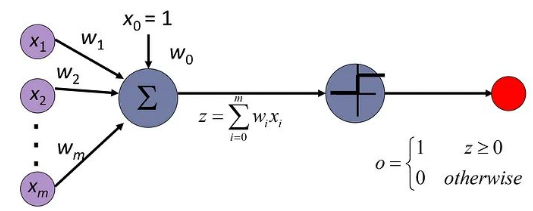
\includegraphics[width=0.45\textwidth]{37.png}
	\caption{Esquema del perceptrón.}
\end{figure}

Los datos entran por $\vec{x}$ (input) y las respuestas salen por $\vec{y}$ (output). El \textbf{bias} $\vec{b}$ es un peso especial que no multiplica a ninguna variable.

\subsection{Arquitecturas: Perceptrón Multicapa (MLP)}

Varias neuronas en paralelo e interconectadas forman arquitecturas que sí resuelven problemas.

\begin{figure}[H]
	\centering
	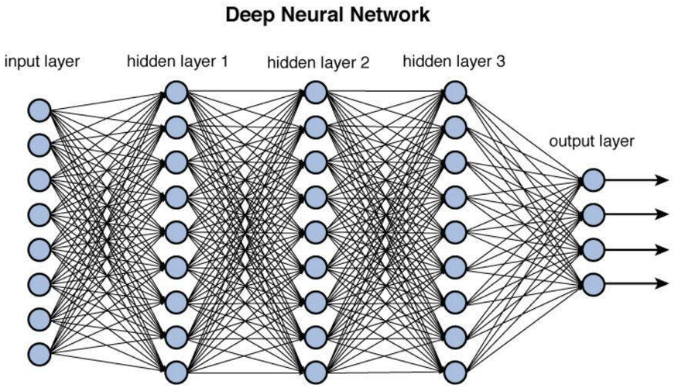
\includegraphics[width=0.5\textwidth]{38.png}
	\caption{Red neuronal feedforward fully-connected.}
\end{figure}

\begin{itemize}
	\item \textbf{Feedforward}: la información va hacia adelante.
	\item \textbf{Fully-connected}: todas las neuronas de una capa conectan con todas las de la siguiente.
	\item Capas: \textbf{input}, \textbf{ocultas} y \textbf{output}.
	\item Más capas en serie = \textbf{deep learning}.
\end{itemize}

\begin{notebox}
	Si no se usan funciones de activación no lineales, apilar neuronas colapsa en una sola transformación lineal. Sin romper la linealidad, no tiene sentido tener múltiples capas.
\end{notebox}

\textbf{Backpropagation} propaga los gradientes de la loss hacia atrás usando la regla de la cadena, indicando cuánto y en qué dirección actualizar cada peso.

\textbf{Tensor}: matrices multidimensionales (estructura base en PyTorch).

% =============================================================
\section{Forward y Backward Propagation}
% =============================================================

\subsection{Entrenamiento}

Se optimizan los parámetros (pesos y biases) para predecir correctamente el conjunto de entrenamiento:
\begin{itemize}
	\item \textbf{Forward}: se evalúa la red y se mide el error con la loss function.
	\item \textbf{Backward}: se corrigen los pesos usando regla de la cadena, derivadas parciales y learning rate.
\end{itemize}

\subsection{Inferencia}

Solo se usa forward propagation (sin actualización de pesos).

\subsection{Vectorización}

La forma matricial del cómputo de una capa es:
\[
	z = W^{\top}\vec{x} + \vec{b}
\]
donde $W$ es la matriz de pesos, $\vec{x}$ el vector de inputs y $\vec{b}$ el vector de biases.

La \textbf{loss function} promedia los errores sobre todas las muestras:
\[
	\mathcal{J}(\hat{y}, y) = \frac{1}{m} \sum_{i=1}^{m} \mathcal{L}(\hat{y}^{(i)}, y^{(i)})
\]

% =============================================================
\section{Funciones de activación}
% =============================================================

\subsection{Complicaciones}

\subsubsection{Vanishing Gradient}
Ocurre en redes profundas cuando los gradientes se vuelven muy pequeños al propagarse hacia las primeras capas. Funciones como sigmoide o tanh tienen derivada casi cero en sus extremos, y multiplicar muchos números pequeños achica aún más el resultado.

\textbf{Consecuencia}: las primeras capas casi no actualizan sus pesos $\Rightarrow$ no aprenden. La red no puede aprender representaciones profundas.

\subsubsection{Zig-Zag}
Si la función de activación tiene salidas siempre positivas (como sigmoide), todos los gradientes de los pesos de esa capa tienen el mismo signo, forzando a todos los pesos a moverse en la misma dirección.

\textbf{Solución}: funciones centradas en cero (como tanh) o normalizar los inputs.

\subsubsection{Dying ReLU}
La derivada de ReLU es exactamente cero para valores negativos, produciendo neuronas muertas que nunca actualizan sus pesos. Puede ser bueno (esparsidad $\Rightarrow$ regularización) o malo (mala inicialización $\Rightarrow$ entrenamiento inútil).

\textbf{Soluciones}: Leaky ReLU, Swish, GELU.

\subsection{Catálogo de Funciones}

\begin{figure}[H]
	\centering
	\begin{minipage}{0.48\textwidth}
		\centering
		
\includegraphics[width=\textwidth]{1.png}
		\caption{Heaviside Step.}
	\end{minipage}\hfill
	\begin{minipage}{0.48\textwidth}
		\centering
		
\includegraphics[width=\textwidth]{2.png}
		\caption{Tanh.}
	\end{minipage}
\end{figure}

\begin{figure}[H]
	\centering
	\begin{minipage}{0.48\textwidth}
		\centering
		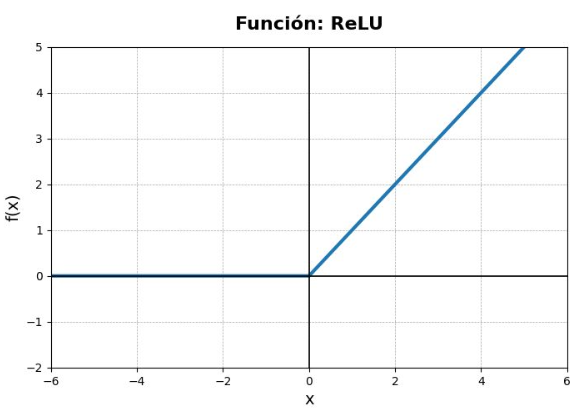
\includegraphics[width=\textwidth]{3.png}
		\caption{ReLU.}
	\end{minipage}\hfill
	\begin{minipage}{0.48\textwidth}
		\centering
		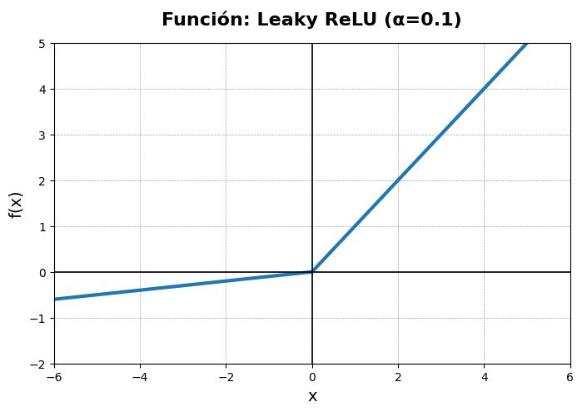
\includegraphics[width=\textwidth]{4.png}
		\caption{Leaky ReLU.}
	\end{minipage}
\end{figure}

\begin{center}
	\begin{tabular}{lll}
		\toprule
		\textbf{Función} & \textbf{Fórmula}                                      & \textbf{Características}                        \\
		\midrule
		Heaviside        & $f(x)=\begin{cases}1 & x\geq0\\0 & x<0\end{cases}$    & Derivada 0 $\Rightarrow$ no sirve para backprop \\[8pt]
		Tanh             & $\dfrac{e^x - e^{-x}}{e^x + e^{-x}}$                  & Centrada en 0, sufre vanishing                  \\[8pt]
		ReLU             & $\max(0,x)$                                           & Barata, no acotada, no centrada en 0            \\[4pt]
		Leaky ReLU       & $\begin{cases}x & x>0\\ \alpha x & x\leq0\end{cases}$ & Evita dying ReLU                                \\[8pt]
		Swish            & $x \cdot \sigma(x)$                                   & Suave, más costosa que ReLU                     \\[4pt]
		GELU             & $x \cdot \Phi(x)$                                     & Buena con Transformers                          \\
		\bottomrule
	\end{tabular}
\end{center}

\begin{figure}[H]
	\centering
	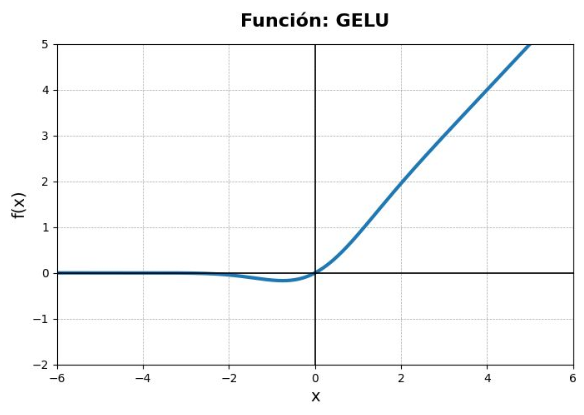
\includegraphics[width=0.5\textwidth]{5.png}
	\caption{Comparación GELU, Swish y otras funciones.}
\end{figure}

\subsection{Softmax}

Toma todo el vector de salidas y lo transforma en probabilidades (entre 0 y 1). Se usa en la última capa para clasificación de clase única:
\[
	f(z)_i = \frac{\exp(z_i)}{\sum_{j=1}^{K} \exp(z_j)}
\]

% =============================================================
\section{Optimización e hiperparámetros}
% =============================================================

\subsection{Loss Landscape}

La loss function suele tener formas irregulares y no se minimiza de forma analítica. Se usan métodos iterativos comenzando con pesos inicializados aleatoriamente.

\subsection{Variantes de Gradient Descent}

\begin{defbox}{Gradient Descent y variantes}
	\begin{itemize}
		\item \textbf{Batch GD (BGD)}: usa todo el dataset por paso. Estable pero costoso en datasets grandes.
		\item \textbf{Stochastic GD (SGD)}: usa una muestra al azar por paso. Barato pero ruidoso.
		\item \textbf{Mini-batch}: agrupa $n$ muestras. Balance entre BGD y SGD.
	\end{itemize}
	\textbf{Época} = pasar todos los datos de entrenamiento (divididos en mini-batches) por la red.
\end{defbox}

\subsection{Problemas de terreno}

\begin{itemize}
	\item \textbf{Ravine}: topología tipo cañón $\Rightarrow$ zig-zag.
	\item \textbf{Mesetas y puntos silla}: pendiente casi cero $\Rightarrow$ SGD no progresa.
\end{itemize}

\textbf{Momentum}: los gradientes ya no son independientes; se acumulan gradientes de pasos anteriores para suavizar la trayectoria.

\subsection{Learning Rate adaptativo}

\begin{center}
	\begin{tabular}{lp{9cm}}
		\toprule
		\textbf{Algoritmo} & \textbf{Idea}                                                                                    \\
		\midrule
		AdaGrad            & LR adaptado por parámetro, inversamente proporcional a la acumulación de gradientes al cuadrado. \\
		RMSProp            & Decaimiento exponencial de la acumulación para olvidar gradientes viejos.                        \\
		ADAM               & Combina momentum con LR adaptativo.                                                              \\
		\bottomrule
	\end{tabular}
\end{center}

\subsection{Schedulers}

Adaptación \emph{temporal} del LR global por épocas:
\begin{itemize}
	\item \textbf{Step decay}: cada $n$ épocas se divide por 2.
	\item \textbf{Exponential decay}: multiplicar por un escalar $<1$ constantemente.
	\item \textbf{Cosine Annealing}: LR sigue una curva de coseno descendente.
	\item \textbf{Reduce on Plateau}: si la loss no mejora en varias épocas, reducir LR a la mitad.
\end{itemize}

\subsection{Hiperparámetros}

Parámetros que se definen de antemano (no los aprende la red). Estrategias de búsqueda:
\begin{enumerate}
	\item Random Search
	\item Grid Search
	\item Optimización Bayesiana
\end{enumerate}

\subsection{Input Scaling}

Las redes son sensibles a los rangos de los inputs. Estandarizar allana el loss landscape y mejora la convergencia.

\begin{figure}[H]
	\centering
	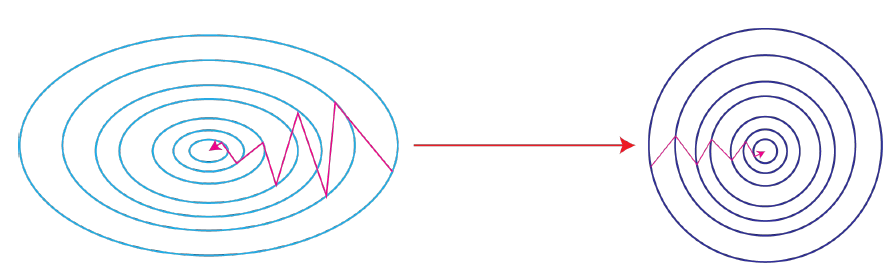
\includegraphics[width=0.55\textwidth]{9.png}
	\caption{Efecto del input scaling en el loss landscape.}
\end{figure}

\subsection{Inicialización de pesos}

La convergencia depende directamente del punto de partida. Una buena inicialización evita vanishing/exploding gradients. Métodos: Random, LeCun, Xavier.

\subsection{Internal Covariate Shift y Batch Normalization}

\begin{defbox}{Internal Covariate Shift}
	Aunque se controle la distribución de entrada, las capas ocultas cambian la distribución de sus salidas durante el entrenamiento, obligando a las capas siguientes a readaptarse constantemente.

	\textbf{Batch Normalization}: normaliza los valores de cada batch antes de ciertas capas, corrigiendo este problema y actuando como regularización.
\end{defbox}

\subsection{Regularización}

\subsubsection{Early Stopping}
Cortar el entrenamiento cuando las curvas de loss de train y validación comienzan a diverger.

\begin{figure}[H]
	\centering
	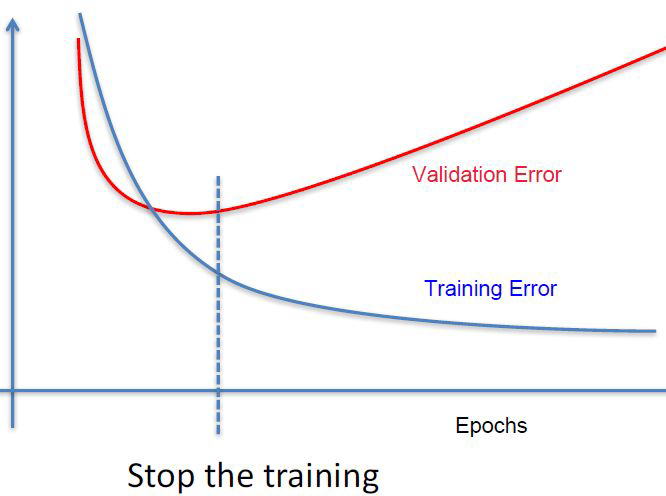
\includegraphics[width=0.45\textwidth]{10.png}
	\caption{Early stopping: punto óptimo antes del sobreajuste.}
\end{figure}

\subsubsection{L1 y L2}
Funciones de presupuesto sumadas a la loss function para restringir los valores de los pesos.

\subsubsection{Dropout}
En cada mini-batch se apagan neuronas al azar, evitando que ciertos patrones sean memorizados. Solo afecta al entrenamiento; en inferencia se usan todas.

\subsubsection{Monitoreo de Gradientes}

\begin{figure}[H]
	\centering
	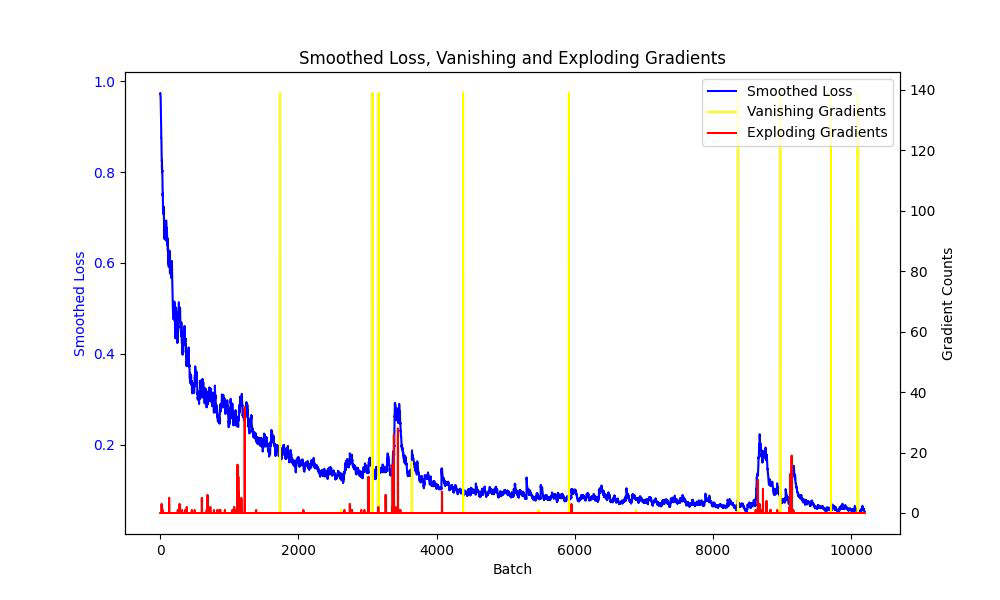
\includegraphics[width=0.55\textwidth]{11.png}
	\caption{Monitoreo: picos en la loss $\leftrightarrow$ exploding gradients; estancamiento $\leftrightarrow$ vanishing.}
\end{figure}

% =============================================================
\section{Redes Neuronales Convolucionales (CNNs)}
% =============================================================

\subsection{Motivación}

En datos no tabulares (imágenes), los píxeles no son independientes entre sí. Una red fully-connected ignora la estructura espacial. Las CNNs explotan la relación entre píxeles vecinos.

Una imagen es una matriz (o tres matrices para RGB) que contiene números.

\subsection{Convolución}

\begin{defbox}{Convolución 2D discreta}
	Operación que toma una imagen $I$ y un kernel $K$ (filtro) pequeño. El kernel se desplaza por la imagen, multiplicando elemento a elemento y sumando:
	\[
		(I * K)[i,j] = \sum_m \sum_n I[i+m,\, j+n] \cdot K[m,n]
	\]
\end{defbox}

\begin{itemize}
	\item \textbf{Padding}: rellenar bordes con ceros para controlar el tamaño de salida.
	\item \textbf{Stride}: el ``tranco'' que da el filtro. Stride grande $\Rightarrow$ salida más chica.
\end{itemize}

\textbf{Fórmula del tamaño de salida}:
\[
	O = \frac{I - K + 2P}{S} + 1
\]

Ejemplo: imagen $28 \times 28$, kernel $3 \times 3$, $P=1$, $S=2$: $O = \frac{28-3+2}{2}+1 = 14$. Salida: $14 \times 14$.

Los filtros (kernels) se inicializan random y se ajustan con backpropagation. La red aprende qué detectar.

\subsection{Pooling}

Resume información de un grupo de píxeles vecinos:
\begin{itemize}
	\item Achica la dimensión (ahorra espacio y cómputo).
	\item Aumenta el campo receptivo.
	\item Da robustez ante traslación.
\end{itemize}

\subsection{Bloque convolucional}

\begin{algbox}{Bloque convolucional estándar}
	\textbf{Convolución} $\longrightarrow$ \textbf{Función de activación} $\longrightarrow$ \textbf{Pooling}

	La convolución es una operación lineal; la no linealidad la aportan la activación y el pooling.
\end{algbox}

\subsection{Ejemplo: parámetros MLP vs CNN}

Para una imagen de $32 \times 32 \times 3$ (color):

\textbf{MLP}: flatten + capa de 128 neuronas + capa de 10 salidas $= (3072 \times 128 + 128) + (128 \times 10 + 10) = 394{,}634$ parámetros.

\textbf{CNN}: conv de 10 filtros $5 \times 5$ + maxpool $2 \times 2$ + conv de 20 filtros $3 \times 3$ $= 760 + 1{,}820 = 2{,}580$ parámetros.

La CNN tiene $\sim$150$\times$ menos parámetros gracias al parameter sharing y la localidad.

% =============================================================
\section{Arquitecturas famosas}
% =============================================================

Todas fueron evaluadas en el \textbf{ImageNet Challenge} (14M imágenes, 22K clases).

\subsection{AlexNet (2012)}

Primera CNN profunda importante para aplicaciones reales. Ganó ImageNet por mucho.

\begin{figure}[H]
	\centering
	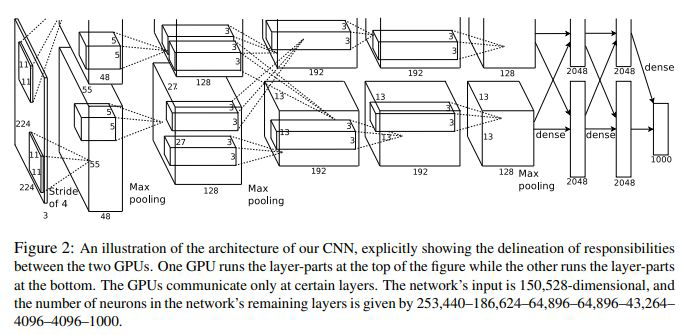
\includegraphics[width=0.7\textwidth]{12.png}
	\caption{Arquitectura AlexNet.}
\end{figure}

Aportes: entrenamiento multi-GPU, capas de normalización, data augmentation, dropout, ensamble de CNNs.

\begin{figure}[H]
	\centering
	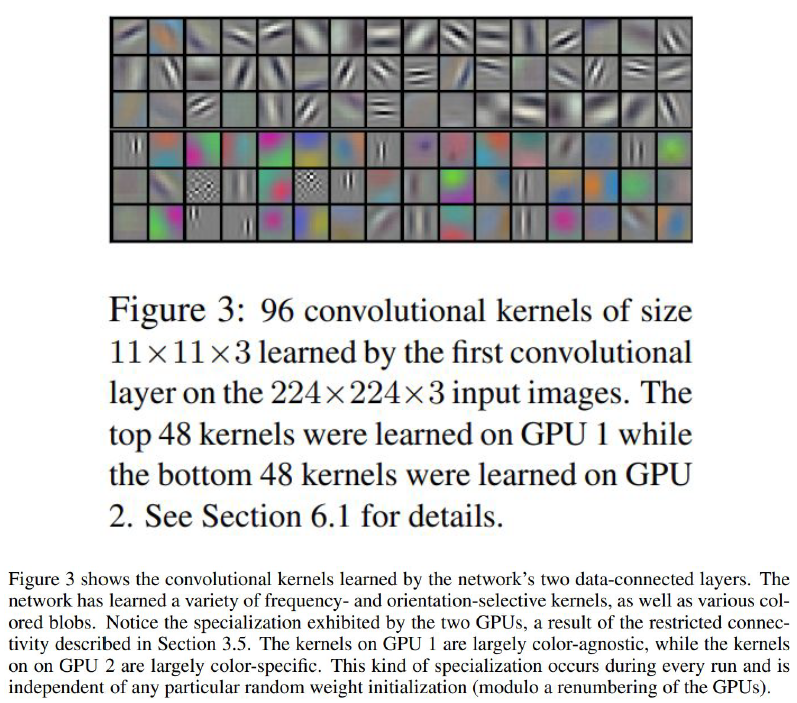
\includegraphics[width=0.55\textwidth]{14.png}
	\caption{Kernels aprendidos por la primera capa convolucional de AlexNet.}
\end{figure}

\subsection{ZFNet (2013)}

Mejoró a AlexNet con ajustes de hiperparámetros. Su contribución principal fue la interpretación visual de lo que aprenden las CNNs.

\subsection{VGG (2014)}

Demostró que usar siempre \textbf{filtros de 3$\times$3 con stride 1} combinados secuencialmente obtiene el mismo campo receptivo que filtros más grandes, con más flexibilidad y menos parámetros. Red profunda y pesada. Buenas representaciones transferibles.

\subsection{GoogLeNet / Inception (2014)}

\begin{defbox}{Inception Module}
	En vez de elegir un tamaño de filtro, se aplican \textbf{distintas convoluciones y max pooling en paralelo}, concatenando las salidas. La red elige el tamaño adecuado.

	\textbf{Convoluciones 1$\times$1}: reducen la cantidad de canales (reducción de dimensionalidad aprendida).

	\textbf{Global Average Pooling}: reemplaza las capas Flatten antes de la clasificación final, reduciendo drásticamente los parámetros.
\end{defbox}

\begin{figure}[H]
	\centering
	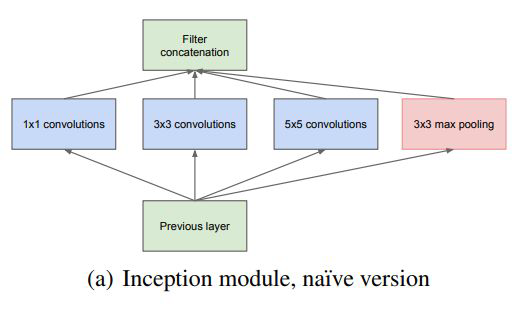
\includegraphics[width=0.6\textwidth]{15.png}
	\caption{Inception Module básico.}
\end{figure}

\begin{figure}[H]
	\centering
	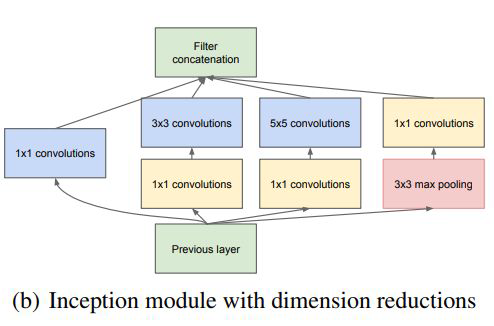
\includegraphics[width=0.6\textwidth]{16.png}
	\caption{Inception Module con convoluciones 1$\times$1 para reducción.}
\end{figure}

22 capas con solo $\sim$5M parámetros (vs.\ $\sim$140M de VGG).

\subsection{ResNet (2015)}

\begin{defbox}{Bloque residual}
	Se agrega una \textbf{skip connection}: el input se bifurca, pasa por convoluciones por un lado y se saltea por otro, sumándose antes de la activación:
	\[
		H(x) = F(x) + x
	\]
	Ventajas:
	\begin{enumerate}
		\item Agregar capas nunca empeora: el bloque puede aprender $F(x)=0$ (identidad).
		\item El gradiente de la skip connection es 1 $\Rightarrow$ mitiga vanishing gradients.
	\end{enumerate}
\end{defbox}

\begin{figure}[H]
	\centering
	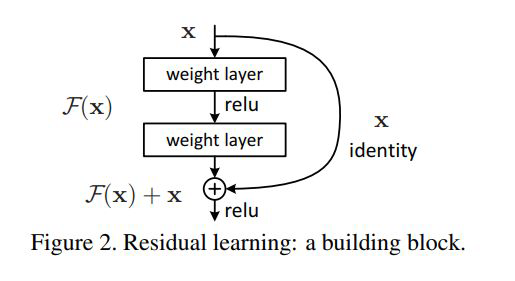
\includegraphics[width=0.5\textwidth]{17.png}
	\caption{Bloque residual con skip connection.}
\end{figure}

Error del 3\% en ImageNet. Terminó efectivamente la competencia.

% =============================================================
\section{Visualización e interpretabilidad de CNNs}
% =============================================================

\subsection{Redes Deconvolucionales (Zeiler \& Fergus)}

\begin{figure}[H]
	\centering
	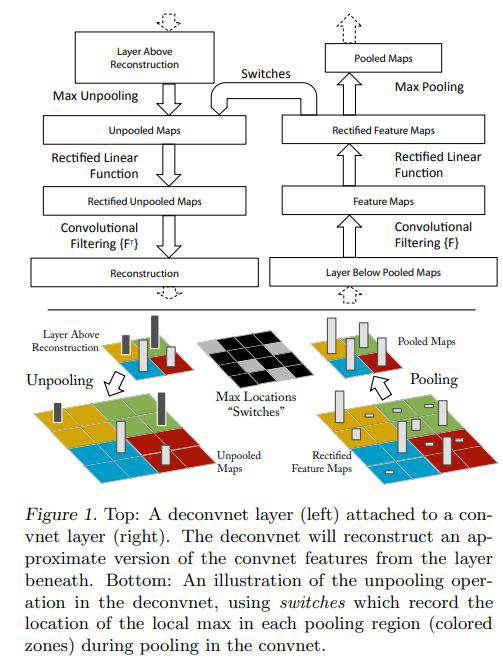
\includegraphics[width=0.5\textwidth]{18.png}
	\caption{Visualización: primeras capas captan patrones generales; últimas capas, detalles refinados.}
\end{figure}

\subsection{Oclusión}

Se tapa una parte de la imagen y se observa cómo afecta la predicción.

\begin{figure}[H]
	\centering
	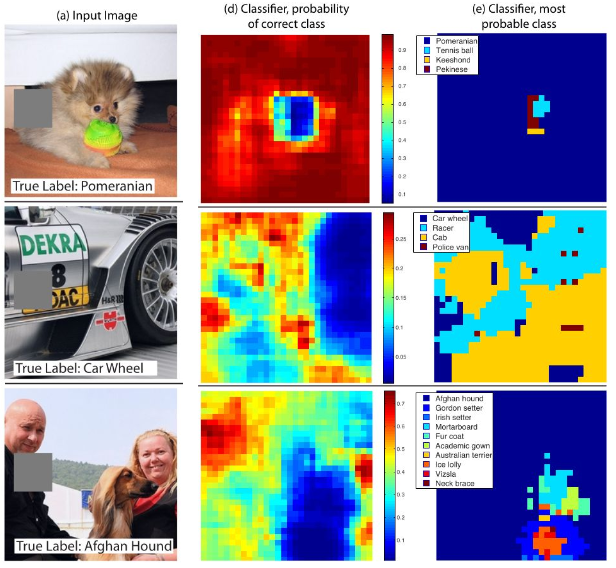
\includegraphics[width=0.5\textwidth]{6.png}
	\caption{Sensibilidad a la oclusión: qué partes de la imagen influyen en la predicción.}
\end{figure}

\subsection{Espacio latente e Image Similarity}

La última capa antes de clasificar codifica imágenes en un espacio de features. Imágenes similares quedan cerca en ese espacio. Se aplican técnicas de reducción de dimensionalidad para visualizar.

\begin{figure}[H]
	\centering
	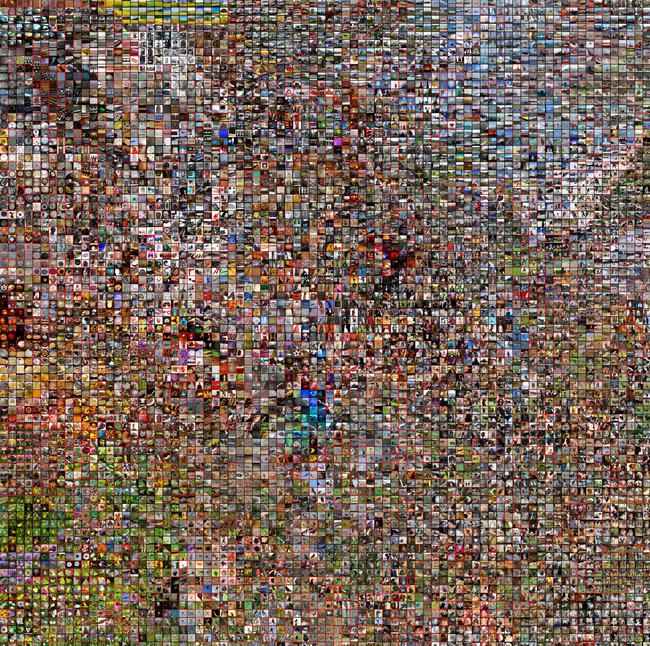
\includegraphics[width=0.5\textwidth]{7.png}
	\caption{Visualización del espacio latente con reducción de dimensionalidad.}
\end{figure}

\subsection{Saliency Maps}

\begin{defbox}{Saliency Maps}
	En una única pasada hacia atrás, se calcula la sensibilidad de la predicción respecto a cada píxel. Los píxeles con mayor gradiente son los más importantes para la clasificación. Se trata al input como variable y a los pesos como fijos.
\end{defbox}

\subsection{Grad-CAM}

En vez de calcular píxel a píxel, calcula la importancia por parches, generando mapas de calor sobre la imagen.

\begin{figure}[H]
	\centering
	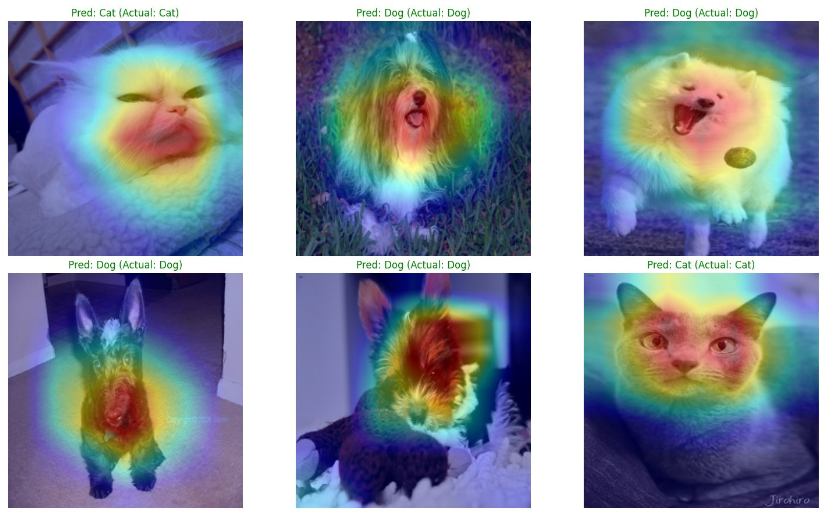
\includegraphics[width=0.55\textwidth]{8.png}
	\caption{Grad-CAM: mapas de calor por parches.}
\end{figure}

\subsection{Ataques Adversarios}

Se busca el mínimo cambio en píxeles para que la red clasifique una imagen como otra clase. Se fija la nueva clase objetivo y se modifica la imagen para maximizar esa probabilidad.

\subsection{Style Transfer}

Transferir el estilo visual de una imagen a otra. Se optimiza una imagen intermedia $I$ minimizando:
\[
	\mathcal{L}_{\text{total}} = \alpha \cdot \mathcal{L}_{\text{content}} + \beta \cdot \mathcal{L}_{\text{style}}
\]

\textbf{Content Loss}: diferencia entre las activaciones de $I$ y la imagen de contenido en capas intermedias de una CNN (e.g.\ VGG). Preserva la estructura.

\textbf{Style Loss}: diferencia entre las \textbf{matrices de Gram} (correlaciones entre feature maps) de $I$ y la imagen de estilo. Capturan texturas y patrones sin importar la posición espacial.

% =============================================================
\section{Transfer Learning}
% =============================================================

\begin{defbox}{Transfer Learning}
	Reutilizar capas preentrenadas en un dataset grande (como ImageNet) para otro problema distinto.
	\begin{itemize}
		\item Entrenar desde cero es muy costoso.
		\item Las primeras capas capturan bordes, formas y texturas útiles para casi cualquier tarea visual.
		\item La última capa FC (específica del problema original) se reemplaza por una nueva.
		\item Se decide cuánto reeentrenar: congelar todo (solo nueva capa) o fine-tuning (algunas capas previas).
	\end{itemize}
\end{defbox}

\begin{figure}[H]
	\centering
	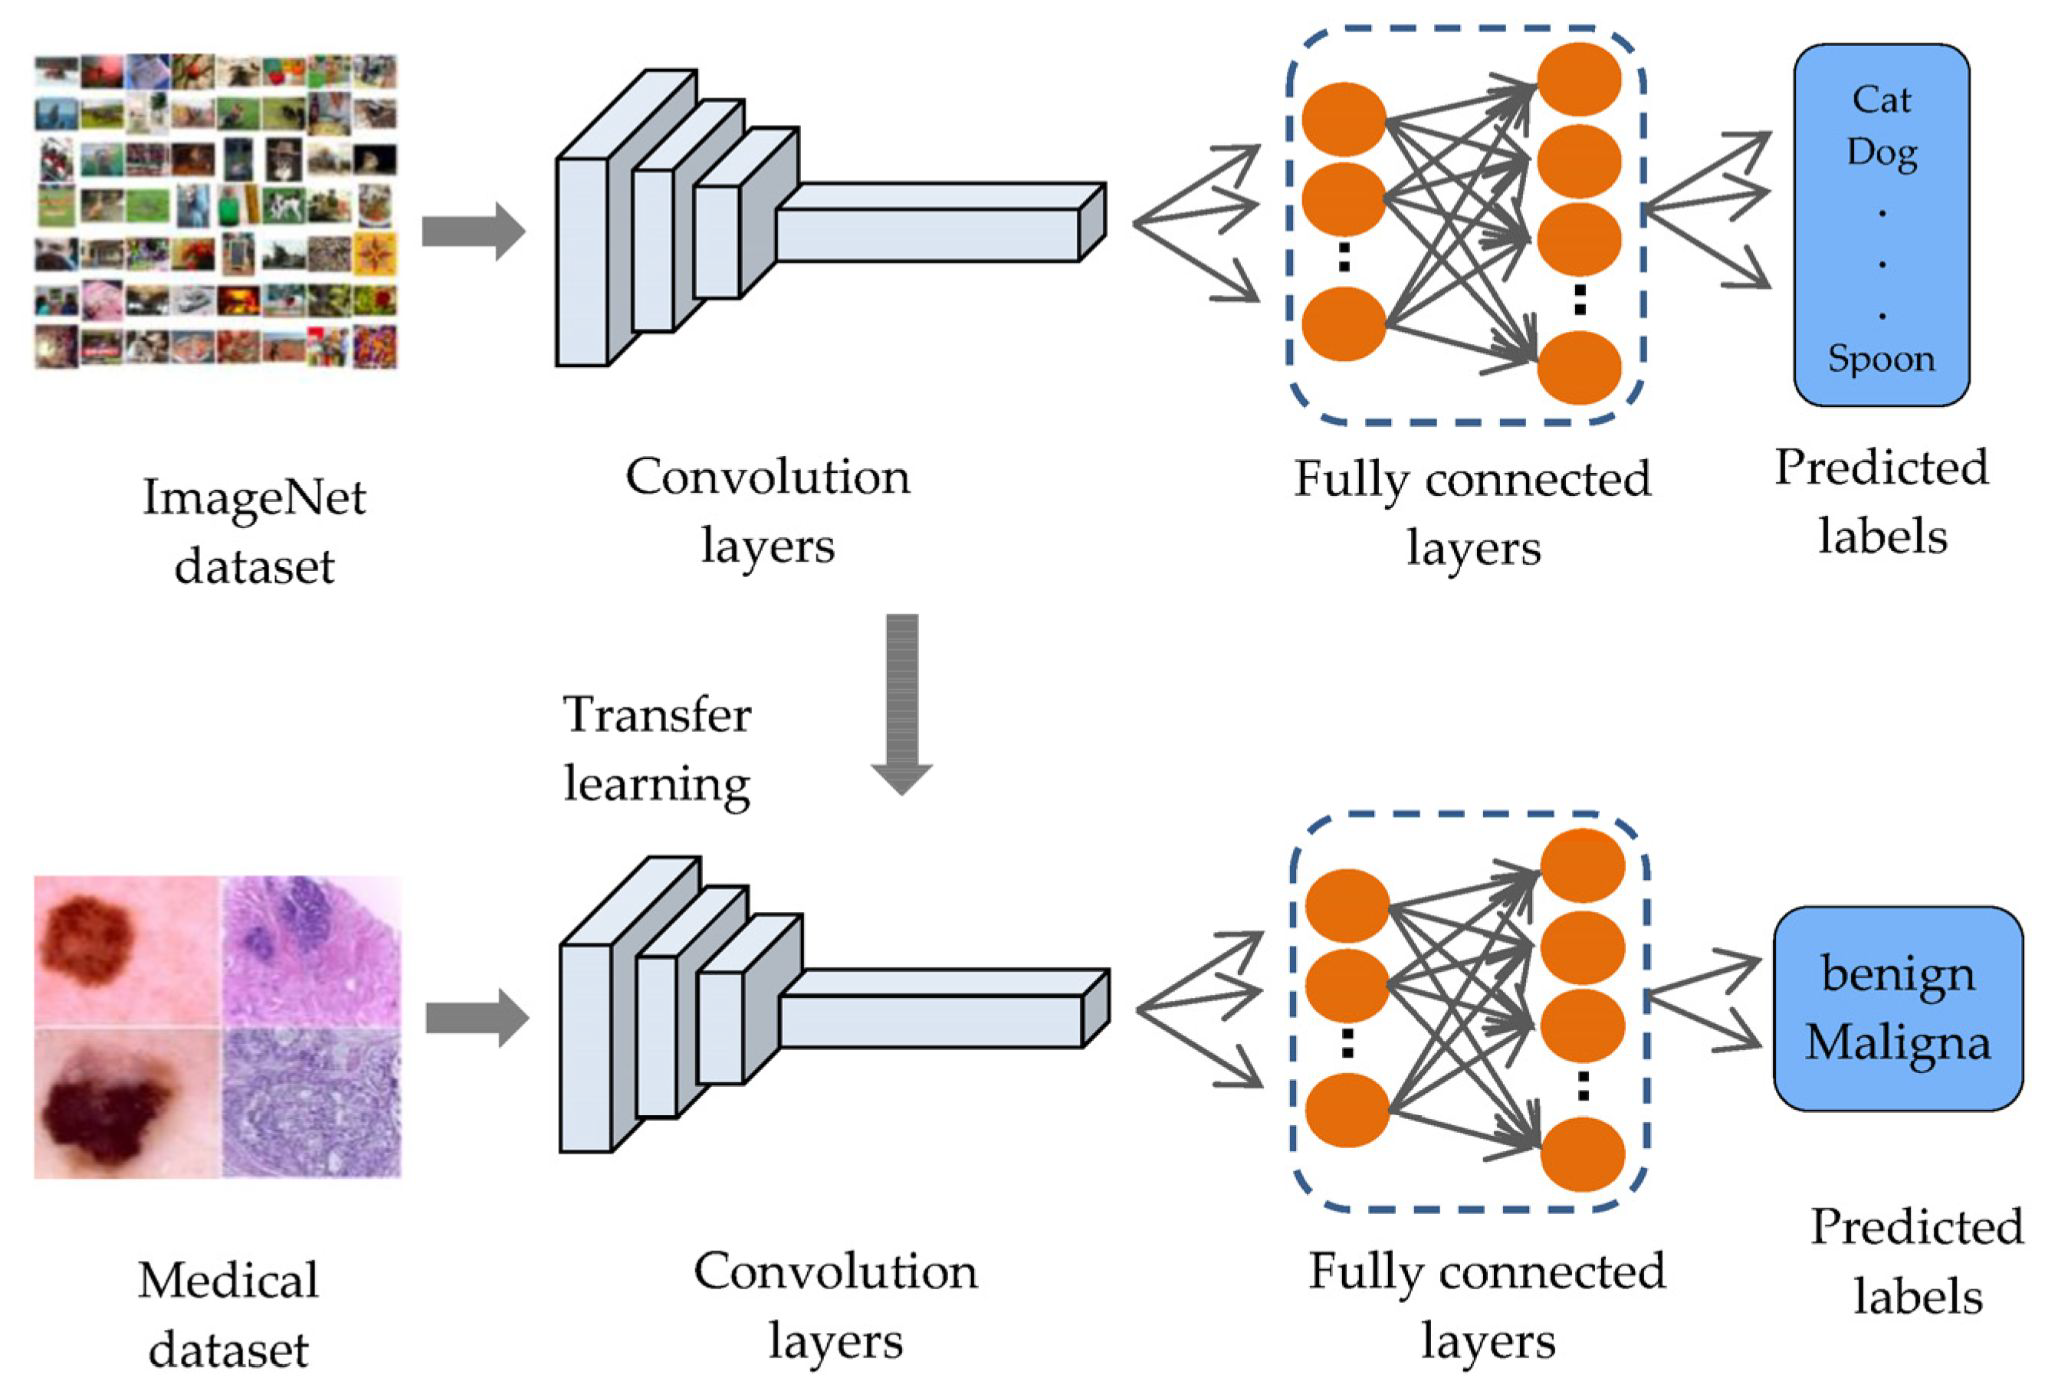
\includegraphics[width=0.65\textwidth]{20.png}
	\caption{Transfer Learning: qué capas reutilizar y qué reemplazar.}
\end{figure}

% =============================================================
\section{Problemas sobre imágenes}
% =============================================================

\subsection{Object Detection}

No solo clasificar objetos, sino \textbf{localizarlos} con una bounding box.

\begin{figure}[H]
	\centering
	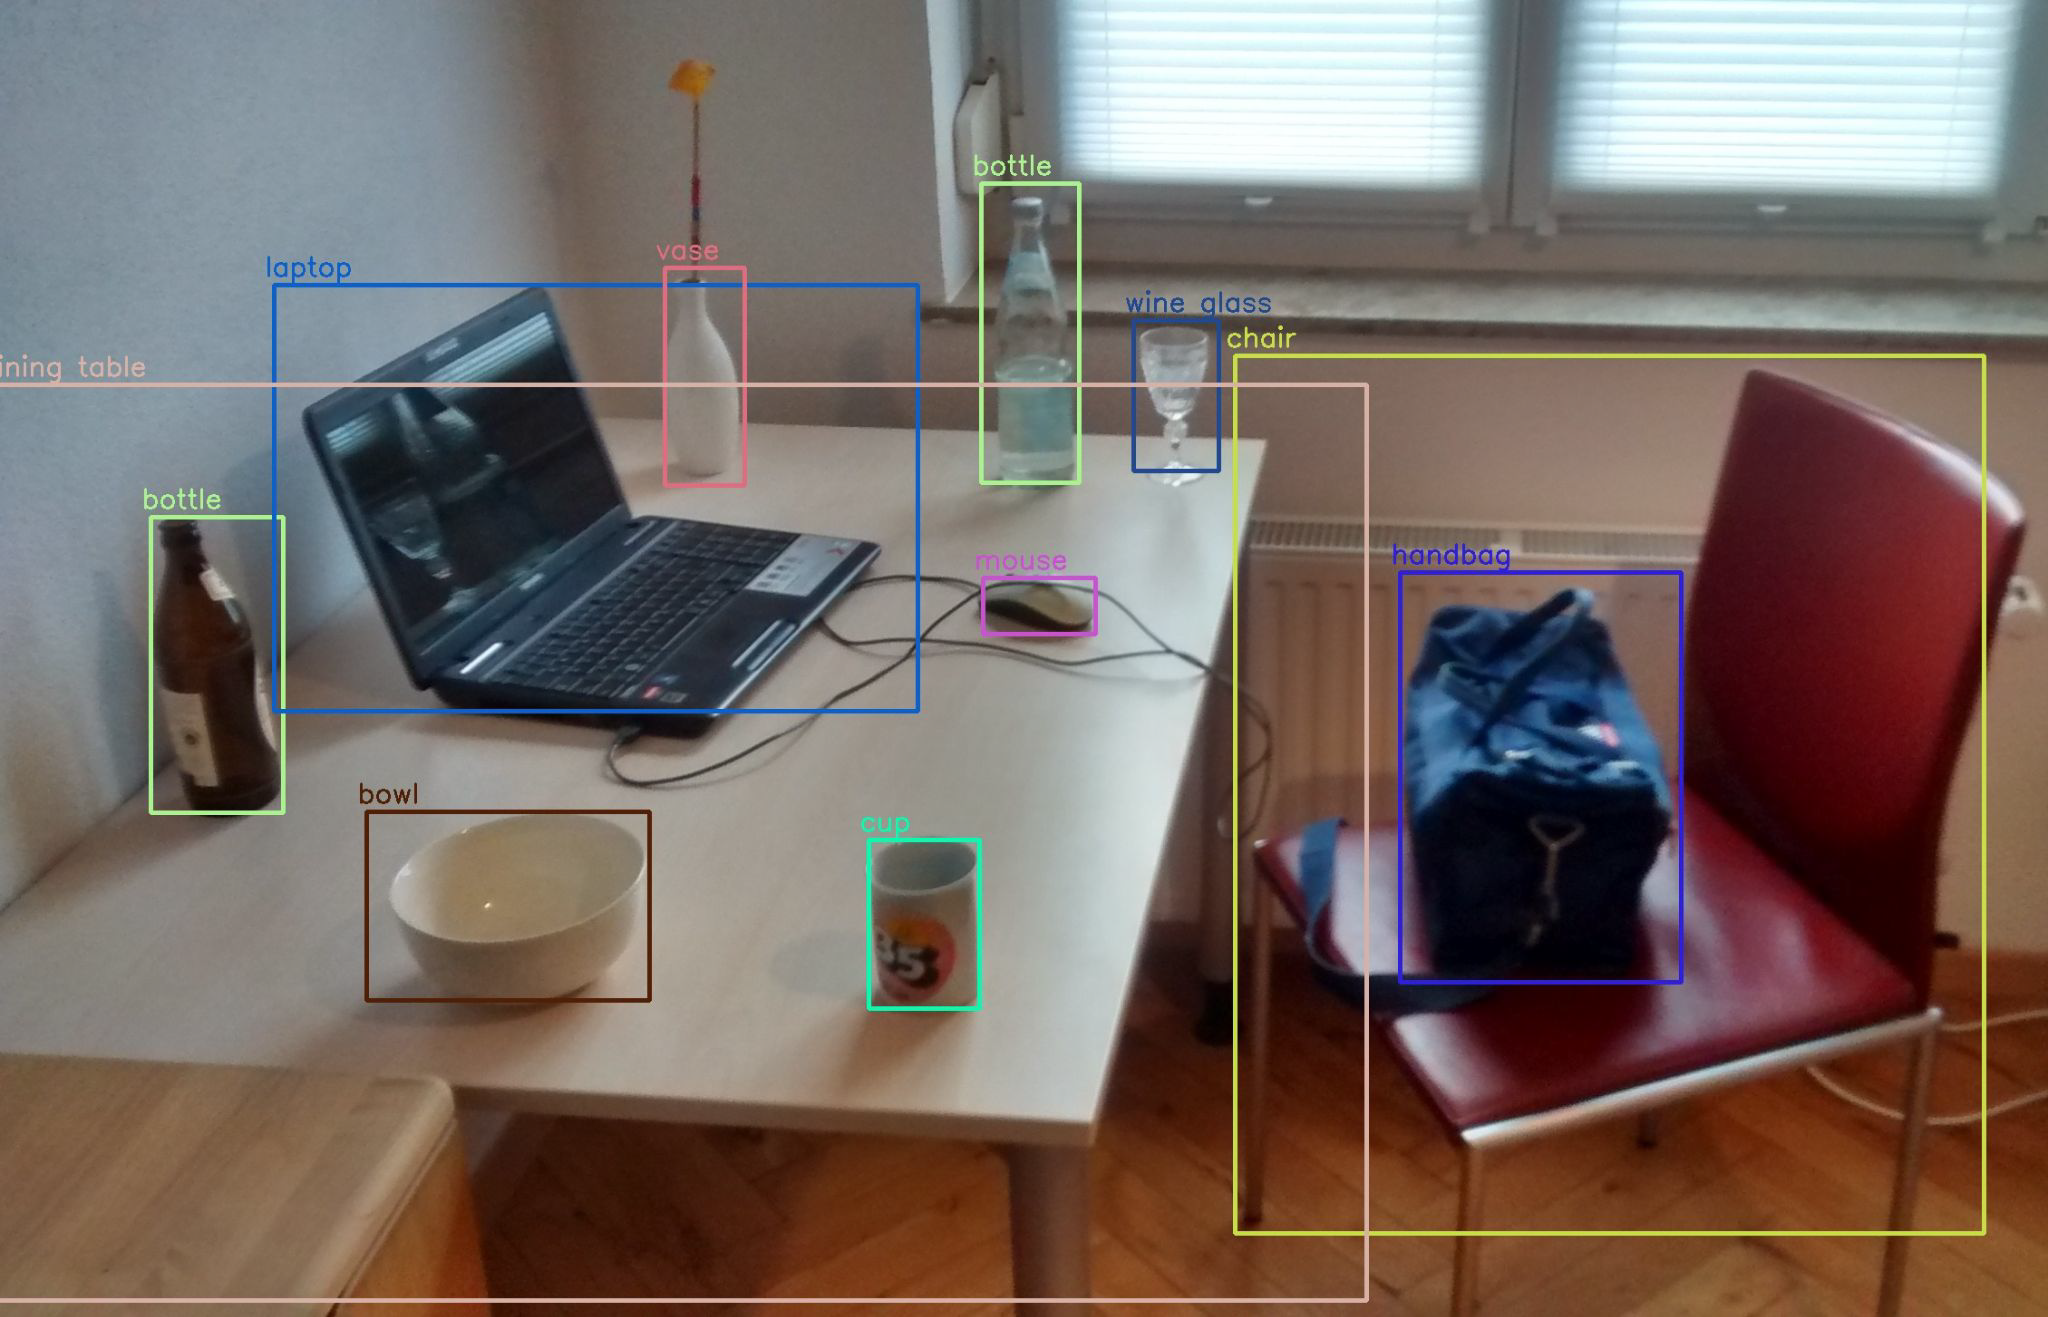
\includegraphics[width=0.6\textwidth]{21.png}
	\caption{Object detection: clasificación + localización.}
\end{figure}

\subsubsection{R-CNN}
Usa \textbf{regiones candidatas} en vez de sliding window. Se hace inferencia sobre cada región.

\begin{figure}[H]
	\centering
	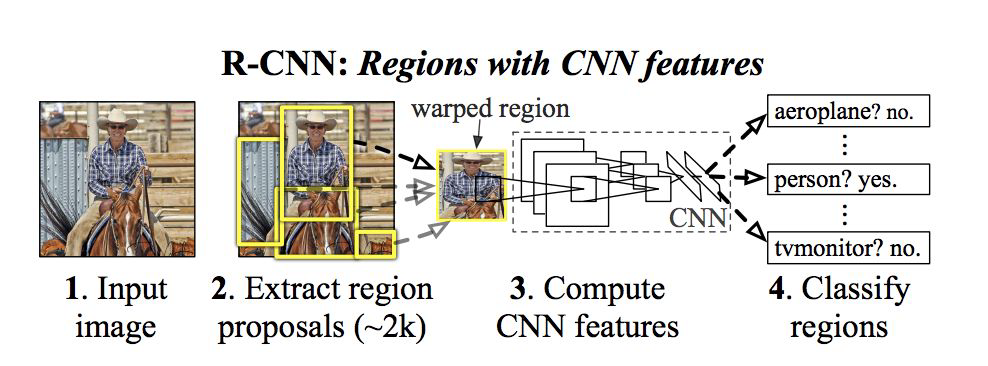
\includegraphics[width=0.65\textwidth]{22.png}
	\caption{Pipeline de R-CNN.}
\end{figure}

\subsubsection{Fast R-CNN}
La imagen entera pasa por la CNN \textbf{una sola vez}, obteniéndose un único feature map. Las regiones candidatas se proyectan sobre ese feature map compartido.

\subsubsection{Faster R-CNN}
Reemplaza el algoritmo externo de regiones por una \textbf{Region Proposal Network} (RPN) que toma el mismo feature map y aprende a proponer regiones.

\subsubsection{YOLO}

\begin{defbox}{YOLO (You Only Look Once)}
	Modelo \textbf{one-stage}: trata la detección como un único problema de regresión. De los píxeles directo a las coordenadas de las cajas y las clases, en una sola pasada.

	\textbf{Loss combinada}: penaliza clasificar mal y poner la caja lejos de la real.

	La imagen se divide en una grilla de $S \times S$ celdas. Cada celda predice $B$ bounding boxes con 5 valores $(x, y, w, h, \text{confidence})$ más $C$ probabilidades de clase. Output total: $S \times S \times (B \times 5 + C)$.

	\textbf{Non-Max Suppression}: muchas celdas detectan el mismo objeto. Se toma la caja con mayor confianza y se descartan las que tengan alta intersección (IoU) con ella.
\end{defbox}

\begin{figure}[H]
	\centering
	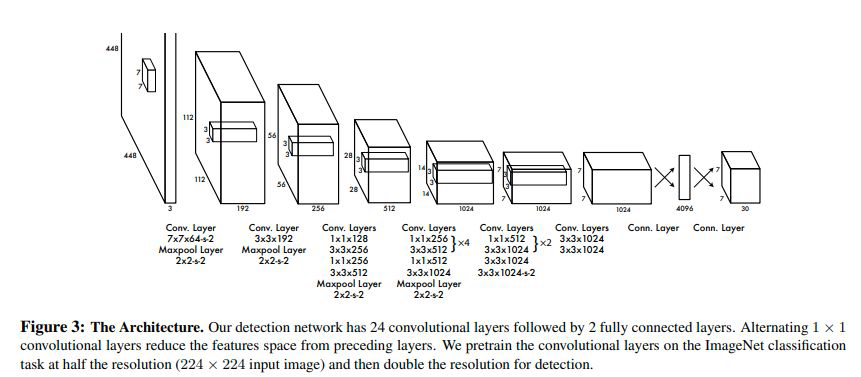
\includegraphics[width=0.55\textwidth]{24.png}
	\caption{Arquitectura YOLO.}
\end{figure}

\begin{figure}[H]
	\centering
	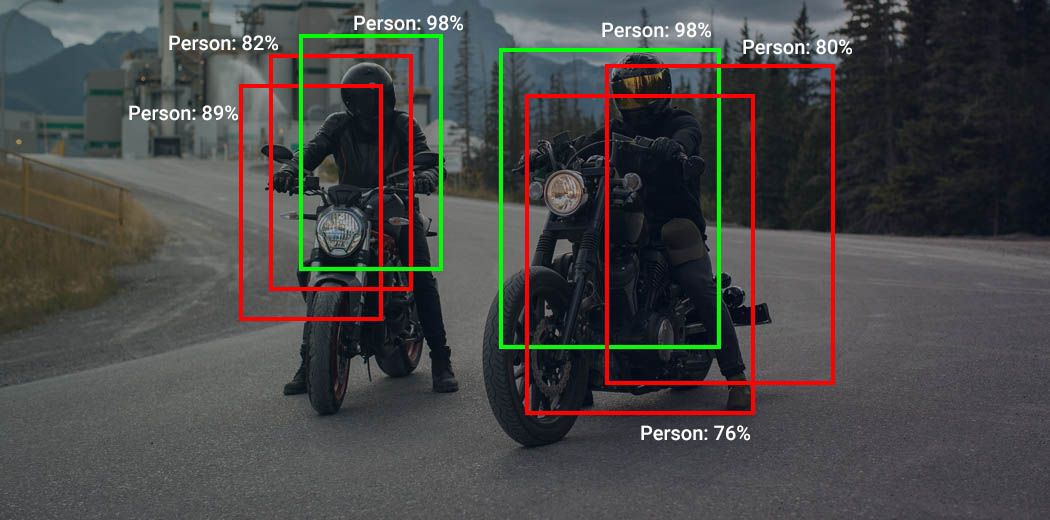
\includegraphics[width=0.45\textwidth]{26.png}
	\caption{Non-Max Suppression.}
\end{figure}

\subsection{Image to Image (I2I)}

Una red puede tener tantas salidas como entradas: recibe una imagen y devuelve otra.

\subsubsection{Autoencoders}

\begin{defbox}{Autoencoder}
	Red que reconstruye su propia entrada:
	\begin{itemize}
		\item \textbf{Encoder}: comprime la imagen hasta una \textbf{representación latente} (downsampling).
		\item \textbf{Decoder}: expande la representación latente hasta reconstruir la imagen original.
		\item \textbf{Loss}: comparación píxel a píxel entre entrada y salida (no requiere etiquetas).
	\end{itemize}
\end{defbox}

\begin{figure}[H]
	\centering
	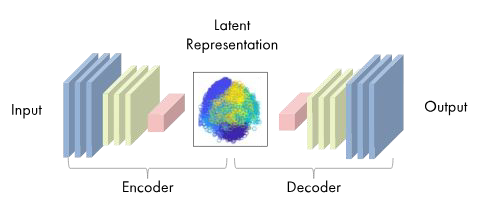
\includegraphics[width=0.7\textwidth]{27.png}
	\caption{Arquitectura de un autoencoder.}
\end{figure}

Usos:
\begin{itemize}
	\item \textbf{Reducción de dimensionalidad}: usar solo el encoder.
	\item \textbf{Image retrieval}: comparar representaciones latentes.
	\item \textbf{Denoising}: la red aprende a eliminar ruido.
	\item \textbf{Inpainting}: reconstruir regiones faltantes de la imagen.
\end{itemize}

\subsubsection{Segmentación semántica}

Clasificar cada píxel de la imagen indicando a qué clase pertenece.

\begin{figure}[H]
	\centering
	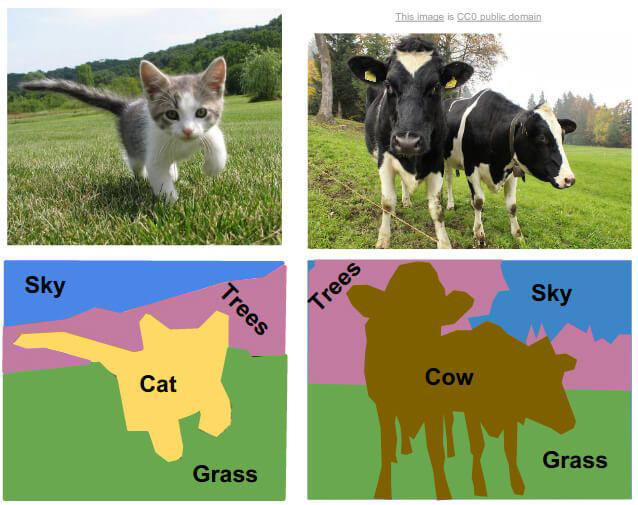
\includegraphics[width=0.55\textwidth]{28.png}
	\caption{Segmentación semántica: cada píxel recibe una clase.}
\end{figure}

Loss functions posibles: Dice Loss, Jaccard Loss, Focal Loss. Se suele preferir \textbf{Dice Loss} sobre cross-entropy porque las clases están muy desbalanceadas (mucho fondo, poco objeto). Dice mide directamente la superposición:
\[
	\text{Dice} = \frac{2|X \cap Y|}{|X| + |Y|}
\]

% =============================================================
\section{Generación de imágenes}
% =============================================================

\subsection{GANs (Generative Adversarial Networks)}

Dos redes entrenadas simultáneamente:
\begin{itemize}
	\item \textbf{Generador}: crea imágenes a partir de ruido.
	\item \textbf{Discriminador}: determina si una imagen es real o generada.
\end{itemize}

\subsection{Modelos de Difusión}

\begin{center}
	\begin{tabular}{lp{9cm}}
		\toprule
		\textbf{Modelo}  & \textbf{Idea}                                                                                              \\
		\midrule
		DDPM             & Sumar ruido progresivamente a una imagen real hasta destruirla. Entrenar una U-Net para deshacer el ruido. \\
		DDIM             & Entrenamiento análogo pero con procedimiento más eficiente.                                                \\
		Stable Diffusion & Difusión en el espacio latente (no en la imagen directamente) para mayor velocidad y estabilidad.          \\
		\bottomrule
	\end{tabular}
\end{center}

\subsection{CLIP}

Conecta texto e imágenes: redes separadas llevan imágenes y texto a espacios latentes distintos, y luego se mapean para unirlos. Permite búsqueda cross-modal.

% =============================================================
\section{Secuencias, texto y NLP}
% =============================================================

\subsection{Dificultades del texto}

Los lenguajes varían en símbolos, orden y separación de palabras. Convertir texto a números no es trivial, a diferencia de las imágenes (que siempre son píxeles).

\subsection{Representaciones de texto}

\subsubsection{Bag-of-Words}

Se olvida del orden y crea un histograma de palabras.

\begin{figure}[H]
	\centering
	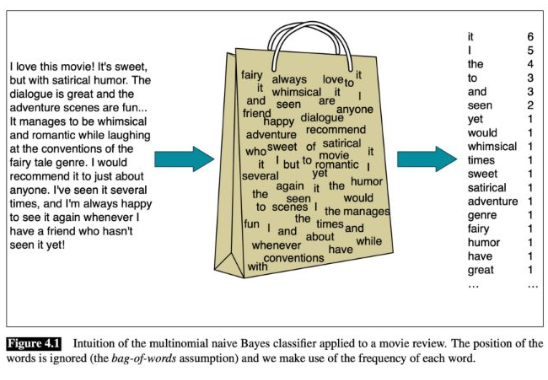
\includegraphics[width=0.45\textwidth]{30.png}
	\caption{Representación Bag-of-Words.}
\end{figure}

Problemas: tantas columnas como palabras, pérdida de orden, ignora contexto y polisemia.

\subsubsection{TF-IDF}

Normalización que le quita peso a palabras muy frecuentes en el corpus. $\text{TF}$ mide frecuencia en el documento; $\text{IDF} = \log(N/n_t)$ penaliza palabras que aparecen en muchos documentos. Producto TF $\times$ IDF da más peso a palabras discriminativas.

\subsubsection{One-Hot Encoding}

Cada token es su propia categoría. Sin semántica: el producto interno entre dos tokens es siempre cero.

\subsubsection{Label Encoding}

Cada token se traduce a un número. Representación simple pero sin semántica real.

\subsection{Word2Vec}

\begin{defbox}{Word Embeddings}
	Llevar palabras a un espacio latente donde las relaciones semánticas se preservan como operaciones vectoriales. Se caracteriza una palabra a partir de las palabras que la rodean.

	Dos modelos:
	\begin{itemize}
		\item \textbf{CBOW}: predecir la palabra del medio a partir de las $n$ anteriores y $n$ posteriores.
		\item \textbf{Skip-Gram}: proceso inverso, predecir las palabras de contexto a partir de la central.
	\end{itemize}
\end{defbox}

\begin{figure}[H]
	\centering
	\begin{minipage}{0.45\textwidth}
		\centering
		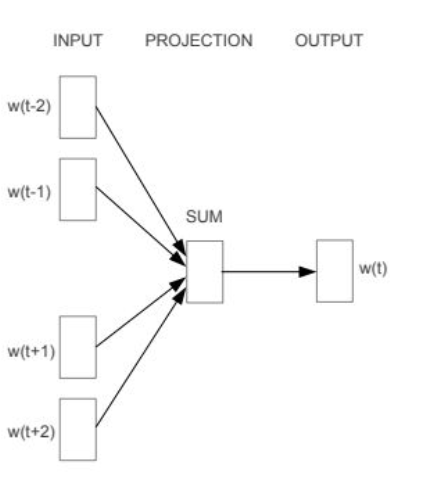
\includegraphics[width=\textwidth]{31.png}
		\caption{Arquitectura CBOW.}
	\end{minipage}\hfill
	\begin{minipage}{0.45\textwidth}
		\centering
		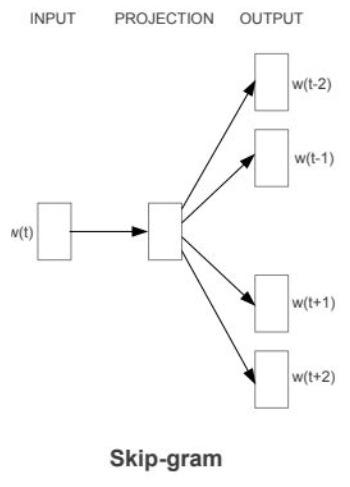
\includegraphics[width=\textwidth]{34.png}
		\caption{Arquitectura Skip-Gram.}
	\end{minipage}
\end{figure}

Proceso CBOW:
\begin{enumerate}
	\item Tomar palabras de contexto (anteriores y posteriores).
	\item Codificar cada una en OHE.
	\item Multiplicar por $W$ para llevar a un espacio latente denso.
	\item Promediar los vectores.
	\item Proyectar con $W'$ a logits de dimensión vocabulario.
	\item Softmax $\Rightarrow$ probabilidades.
	\item Comparar con ground truth y actualizar $W$ y $W'$.
\end{enumerate}

\begin{figure}[H]
	\centering
	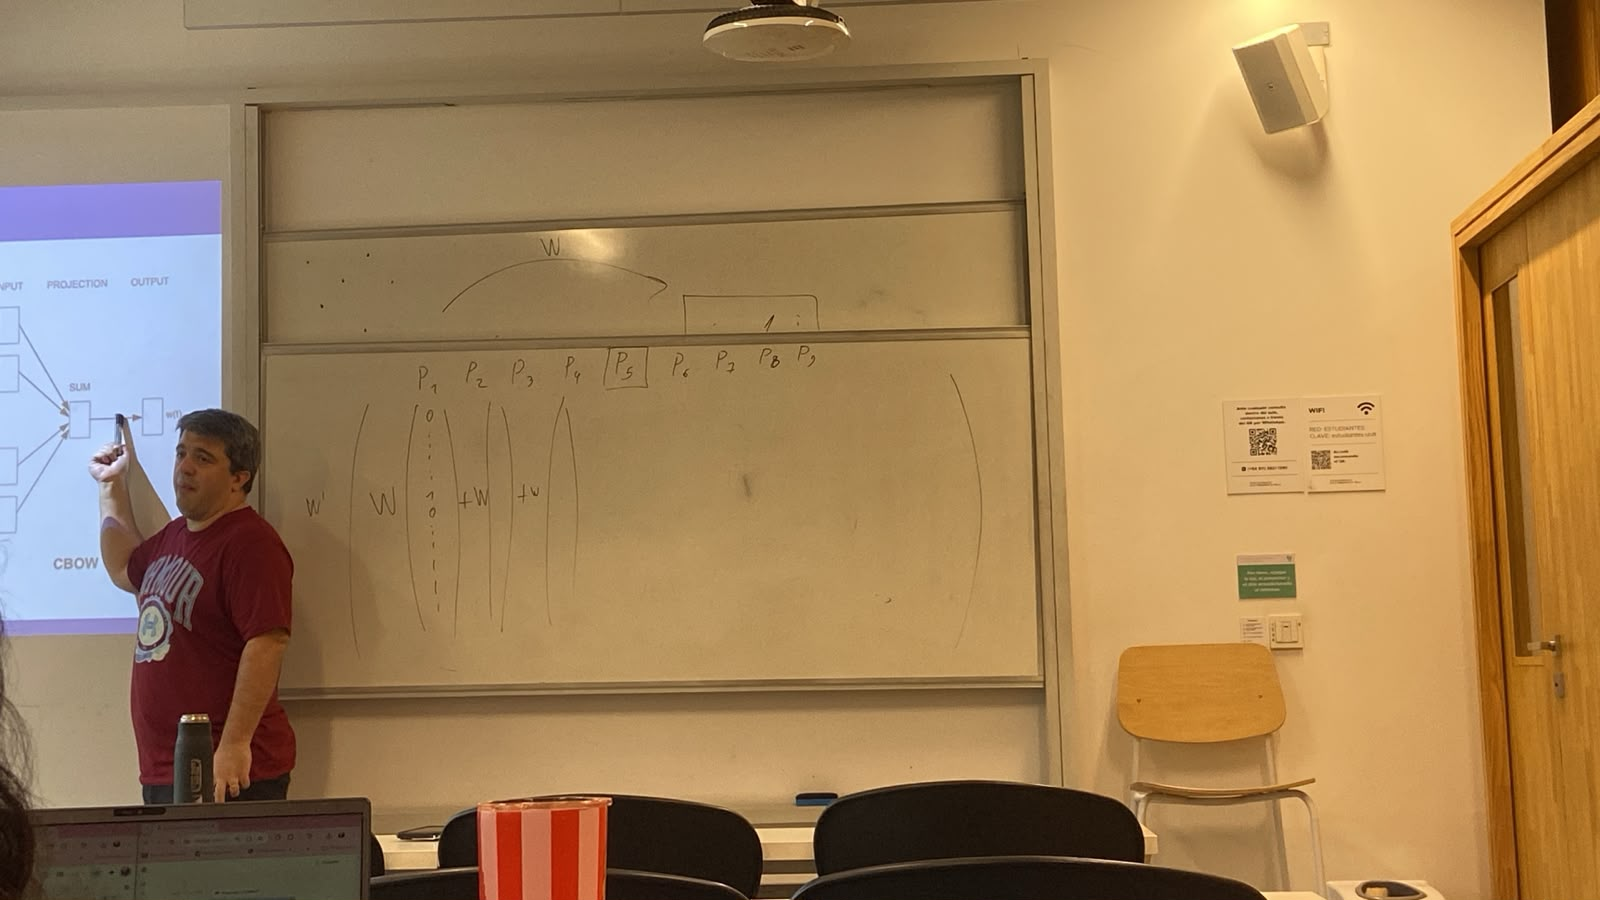
\includegraphics[width=0.6\textwidth]{33.png}
	\caption{Pipeline completo de CBOW.}
\end{figure}

\textbf{Analogías vectoriales}: $v_{\text{madrid}} \approx v_{\text{paris}} - v_{\text{francia}} + v_{\text{españa}}$. Se busca la palabra cuyo vector sea más cercano al resultado.

\textbf{Product2Vec}: misma idea aplicada a secuencias de productos para encontrar productos similares.

\subsection{Language Models}

Buscan predecir la siguiente palabra en una secuencia. Se reduce a un problema de clasificación sobre todo el vocabulario.

% =============================================================
\section{Redes Neuronales Recurrentes (RNNs)}
% =============================================================

\begin{defbox}{RNN}
	Permiten procesar secuencias de tamaño variable (a diferencia de las redes feedforward con inputs fijos). El \textbf{bloque recurrente} recibe el input $x_t$ y una retroalimentación del resultado anterior:
	\[
		h_t = \sigma(W_1 x_t + W_2 h_{t-1})
	\]
	El hidden state $h_t$ codifica información de todas las palabras procesadas anteriormente. La retroalimentación se corta en algún punto.
\end{defbox}

\textbf{Backpropagation Through Time (BPTT)}: al desenrollar la RNN, los gradientes dependen de la exponenciación de la matriz de pesos $W_{hh}$. Multiplicar muchas veces la misma matriz hace que los gradientes se desvanezcan (o exploten). En la práctica, secuencias de 25--30 pasos ya sufren este problema $\Rightarrow$ las RNNs no pueden aprender dependencias lejanas.

% =============================================================
\section{LSTM, Seq2Seq y Attention}
% =============================================================

\subsection{LSTM (Long Short-Term Memory)}

\begin{defbox}{LSTM}
	Tipo de RNN que soluciona el problema de que el gradiente se desvanece para aprender dependencias lejanas.

	Dos vectores de estado:
	\begin{itemize}
		\item \textbf{Hidden state} $\vec{h}$: memoria a corto plazo del contexto actual.
		\item \textbf{Cell state} $\vec{c}$: memoria a largo plazo que pasa información sin desvanecerse.
	\end{itemize}

	\textbf{Gates} (vectores que controlan el flujo de información):
	\begin{itemize}
		\item \textbf{Forget Gate}: decide qué \emph{borrar} del cell state. Sigmoide: 0 = olvidar, 1 = recordar.
		\item \textbf{Input Gate}: decide \emph{cuánto} de lo nuevo se escribe en $c$ (sigmoide) y \emph{qué} (tanh).
		\item \textbf{Output Gate}: decide cuánto del cell state se expone como salida $h_t$.
	\end{itemize}
\end{defbox}

\begin{figure}[H]
	\centering
	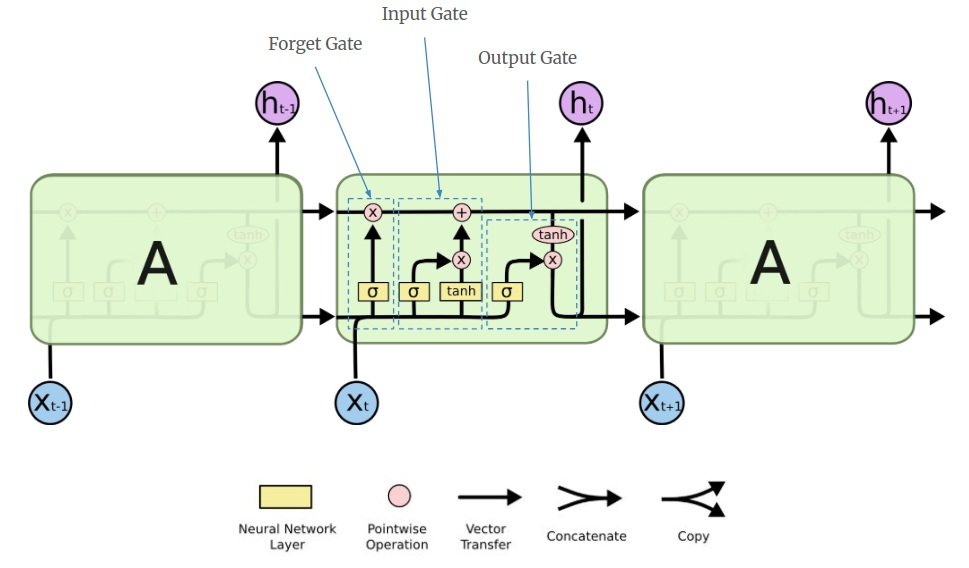
\includegraphics[width=0.6\textwidth]{35.png}
	\caption{Arquitectura interna de una celda LSTM.}
\end{figure}

El ``+'' en el cómputo de $C_t$ permite que la información fluya sin desvanecerse (análogo a las skip connections de ResNet). Si forget gate = 1 e input gate = 0, el cell state fluye intacto.

\subsection{BiLSTM}

Misma idea que LSTM pero en \textbf{ambas direcciones}: izquierda a derecha y derecha a izquierda, obteniendo el doble de hidden states. Captura contexto de ambos lados de cada token.

\subsection{GRU (Gated Recurrent Unit)}

Versión simplificada de LSTM: combina $c$ y $h$ en un solo vector, y fusiona forget e input gates. Menos parámetros, rendimiento similar.

\subsection{Limitaciones de LSTM/BiLSTM}

\begin{itemize}
	\item Procesan secuencialmente $\Rightarrow$ \textbf{no paralelizables}.
	\item Memoria a largo plazo limitada (mejor que RNN, pero no infinita).
	\item Resumen todo en un vector fijo final.
\end{itemize}

\subsection{Seq2Seq}

\begin{defbox}{Seq2Seq}
	Toma secuencias para generar otras secuencias (e.g.\ traducción). Usa dos LSTMs:
	\begin{itemize}
		\item \textbf{Encoder}: procesa la secuencia de entrada y genera una representación.
		\item \textbf{Decoder}: genera la secuencia de salida a partir de esa representación.
	\end{itemize}
	En entrenamiento se usa \textbf{teacher forcing}: en cada paso del decoder se ingresa la palabra correcta aunque no haya sido la predicha.
\end{defbox}

\begin{figure}[H]
	\centering
	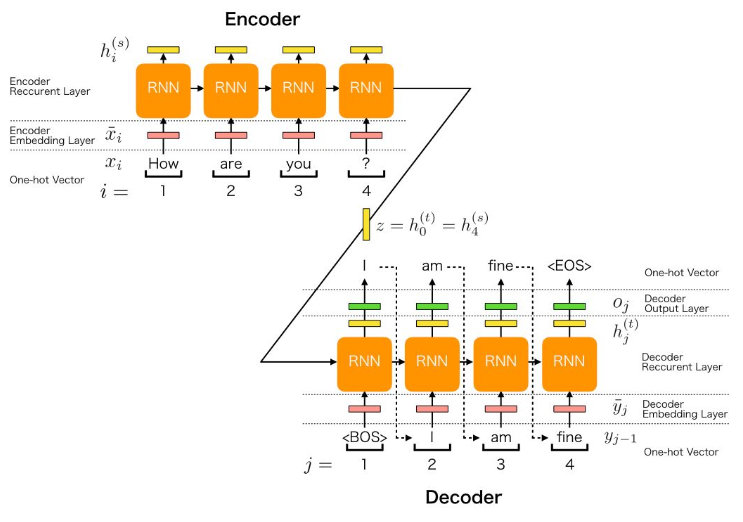
\includegraphics[width=0.7\textwidth]{36.png}
	\caption{Arquitectura Seq2Seq con encoder-decoder.}
\end{figure}

\subsection{Attention}

Mecanismo que permite al decoder ``mirar'' todas las posiciones de la secuencia de entrada (no solo el último hidden state del encoder), asignando pesos de importancia a cada posición según su relevancia para la palabra que se está generando.

Supongamos que estamos generando la tercera palabra de la traducción. Ya tenemos todos los hidden states $h_i$ del encoder y el estado $s_{t-1}$ del decoder. Se calculan \textbf{scores de atención} para cada $h_i$:
\[
	e_{t,i} = v_a^\top \tanh(W_a s_{t-1} + U_a h_i)
\]
donde $v_a, W_a, U_a$ son pesos aprendibles. Luego se pasan por softmax para obtener pesos $\alpha_{t,i}$ y se calcula el \textbf{vector de contexto}:
\[
	c_t = \sum_i \alpha_{t,i} \, h_i
\]

Este vector $c_t$ se concatena con la entrada del decoder en el paso $t$. La semántica es: ``para dar la siguiente palabra, enfocate en esta parte de la frase original''.

\begin{notebox}
	\textbf{Cuello de botella Seq2Seq}: sin Attention, toda la información de la frase de entrada se comprime en un único vector $h$ final del encoder. Funciona para frases cortas, pero no para párrafos. Attention resuelve esto dejando al decoder ver todos los $h_i$ intermedios.
\end{notebox}

% =============================================================
\section{Transformers}
% =============================================================

\subsection{Problema de secuencialidad de las RNNs}

Aunque Attention resolvió el cuello de botella en la representación, las RNNs siguen siendo \textbf{inherentemente secuenciales}: para conocer el estado en el paso 50, primero hay que computar los 49 anteriores. No son paralelizables. Las CNNs no tenían este problema y por eso entre 2012--2016 aprovecharon mejor los avances en hardware.

\subsection{Attention Is All You Need (2017)}

El paper de Vaswani et al.\ propuso el \textbf{Transformer}: no es necesario usar RNNs. El mismo mecanismo de atención que relacionaba encoder con decoder se puede usar como ladrillo fundamental.

\subsection{Self-Attention}

En la atención clásica (Bahdanau), la atención era \textbf{cruzada} entre la frase del decoder y la del encoder. En \textbf{Self-Attention}, las palabras de una misma oración se prestan atención a sí mismas para construir una representación rica.

\subsection{Scaled Dot-Product Attention}

\begin{defbox}{Scaled Dot-Product Attention}
	Paso a paso:
	\begin{enumerate}
		\item Secuencia de palabras $w_i$.
		\item Convertir a embeddings: $x_i = E \, w_i$.
		\item Transformar cada embedding en su \textbf{Query} $q_i = Q x_i$, \textbf{Key} $k_i = K x_i$ y \textbf{Value} $v_i = V x_i$.
		\item Calcular similaridades: $e_{ij} = \dfrac{q_i^\top k_j}{\sqrt{d_k}}$.
		\item Normalizar con softmax: $\alpha_{ij} = \dfrac{\exp(e_{ij})}{\sum_{j'} \exp(e_{ij'})}$.
		\item Salida: suma ponderada de values: $o_i = \sum_j \alpha_{ij} \, v_j$.
	\end{enumerate}

	En forma matricial:
	\[
		\text{Attention}(Q,K,V) = \text{softmax}\!\left(\frac{QK^\top}{\sqrt{d_k}}\right) V
	\]
\end{defbox}

\textbf{Intuición}: es como una \emph{lookup table suavizada}. En un diccionario, se tiene una query $q$, se busca la key $k$ exacta y se toma su value $v$. En self-attention, la query tiene correspondencia parcial con varias keys y se toma el promedio ponderado de los values.

\subsection{Preguntas Clave del Mecanismo}

\begin{itemize}
	\item \textbf{¿De dónde salen Q, K, V?} Son matrices de pesos aprendibles. Se inicializan random y se ajustan con backpropagation.
	\item \textbf{¿Por qué dividir por $\sqrt{d_k}$?} Cuando la dimensión es grande, el producto interno crece mucho. La división estabiliza las cuentas (de ahí ``scaled'').
	\item \textbf{¿Por qué aprender Q y K por separado?} La multiplicación $q_i^\top k_j$ es una \textbf{low-rank factorization} de la matriz de scores $e_{ij}$. Más eficiente computacionalmente y obliga a un cuello de botella en la representación.
	\item \textbf{¿Qué rompe la linealidad?} La softmax rompe un poco, pero el objetivo principal de no linealidad viene de las capas feed-forward con funciones de activación que se agregan después.
\end{itemize}

\subsection{Masked Attention}

En el decoder, las palabras se generan de forma online: al tener la palabra $t$, no se conoce la $t+1$. Se \textbf{enmascaran} los scores de palabras futuras fijándolos en $-\infty$ para que la softmax les asigne peso cero.

\subsection{Positional Encoding}

\begin{defbox}{Positional Encoding}
	Sin recurrencia, self-attention procesa todas las palabras en paralelo y pierde la noción de orden (se vuelve un bag-of-words). La solución: \textbf{sumar un vector de posición} a cada embedding.

	El paper original usó funciones de senos y cosenos de distintas frecuencias:
	\[
		PE_{(pos, 2i)} = \sin\!\left(\frac{pos}{10000^{2i/d}}\right), \quad
		PE_{(pos, 2i+1)} = \cos\!\left(\frac{pos}{10000^{2i/d}}\right)
	\]

	Evolución posterior: Positional Encoding aprendible $\rightarrow$ Relative PE $\rightarrow$ Rotary PE (RoPE).
\end{defbox}

\subsection{Multi-Head Attention}

\begin{defbox}{Multi-Head Attention}
	Análogo a tener múltiples filtros en una CNN: sobre las mismas palabras se quieren aprender \textbf{diferentes representaciones}. Una cabeza puede aprender a reconocer entidades (países, personas), otra a relacionar verbo y sujeto.

	Se ejecutan $h$ mecanismos de atención en paralelo, cada uno con sus propias matrices $Q_i, K_i, V_i$. Las salidas se concatenan y se proyectan con una capa lineal.

	Son computacionalmente muy eficientes.
\end{defbox}

\subsection{Arquitectura del Transformer}

Sigue teniendo \textbf{encoder} y \textbf{decoder}, pero sin RNNs:
\begin{itemize}
	\item El encoder tiene capas de \textbf{self-attention} + feed-forward.
	\item El decoder tiene capas de \textbf{masked self-attention} + \textbf{cross-attention} (con el encoder) + feed-forward.
	\item \textbf{Add \& Norm}: después de cada bloque hay una conexión residual (como ResNet) y Layer Normalization (reemplazo de BatchNorm). Ayudan al flujo de gradientes y aceleran convergencia.
\end{itemize}

Ya en el trabajo original se consiguieron resultados estado del arte en traducción automática con mucho menos entrenamiento que los modelos previos (LSTMs).

\subsection{BERT vs GPT}

\begin{center}
	\begin{tabular}{lp{5.5cm}p{5.5cm}}
		\toprule
		                           & \textbf{BERT (2018, Google)}                                                 & \textbf{GPT (2018, OpenAI)}          \\
		\midrule
		\textbf{Parte usada}       & Solo encoder                                                                 & Solo decoder                         \\
		\textbf{Dirección}         & Bidireccional                                                                & Autorregresivo (izquierda a derecha) \\
		\textbf{Uso}               & Clasificación, NER, Sentiment Analysis (requiere fine-tuning)                & Generación de texto                  \\
		\textbf{Pre-entrenamiento} & Masked Language Model (predecir palabras ocultas) + Next Sentence Prediction & Predecir la siguiente palabra        \\
		\bottomrule
	\end{tabular}
\end{center}

\subsection{Evolución de GPT}

\begin{itemize}
	\item \textbf{GPT-1 (2018)}: El foco era resolver problemas de NLP con fine-tuning. Perdía contra BERT.
	\item \textbf{GPT-2 (2019)}: Foco en resolver tareas NLP sin fine-tuning (\textbf{zero-shot learning}).
	\item \textbf{GPT-3 (2020)}: Foco completamente en el Language Model y todo lo que puede resolver sin ajuste adicional.
\end{itemize}

\subsection{InstructGPT y alineación}

\begin{defbox}{InstructGPT y RLHF}
	Un Language Model bueno genera secuencias gramaticalmente correctas, pero puede no estar \textbf{alineado} con la intención del usuario. Ejemplo: ante una pregunta, GPT-3 completaba con opciones multiple choice como si fuera un examen.

	\textbf{InstructGPT} resolvió esto con \textbf{Reinforcement Learning from Human Feedback (RLHF)}:
	\begin{enumerate}
		\item Se entrena un modelo de recompensa con preferencias humanas.
		\item Se usa RL para ajustar el LLM y que maximice esa recompensa.
	\end{enumerate}

	ChatGPT (nov.\ 2022) usó GPT-3 como backbone + técnicas de alineación para ser conversacional.
\end{defbox}

\subsection{LLMs: Más que un predictor de palabras}

El backbone de un LLM sigue siendo el decoder de un Transformer, pero hay componentes adicionales:
\begin{itemize}
	\item \textbf{Tokenizers}: cómo se segmenta el texto en tokens.
	\item \textbf{Data}: calidad y cantidad de datos de entrenamiento.
	\item \textbf{SFT y RLHF}: Supervised Fine-Tuning y alineación con feedback humano.
	\item Optimizaciones de cómputo.
\end{itemize}

\subsection{Vision Transformers (ViT)}

\begin{defbox}{ViT (2021)}
	Idea análoga a ``Attention Is All You Need'' pero para imágenes: no hacen falta CNNs. Se parte la imagen en \textbf{parches} y se aplican mecanismos de atención entre ellos.

	Buenos resultados pero con tiempos de cómputo altos (prohibitivos para resoluciones altas). La batalla CNN vs ViT sigue abierta para visión, a diferencia de texto donde el Transformer ganó claramente.
\end{defbox}

\subsection{Tipos de Transformers (resumen)}

\begin{center}
	\begin{tabular}{llp{6cm}}
		\toprule
		\textbf{Tipo}   & \textbf{Ejemplo} & \textbf{Uso}                                     \\
		\midrule
		Encoder-Only    & BERT             & Comprender texto: clasificación, sentiment, NER  \\
		Encoder-Decoder & T5, Transformer  & Seq2Seq: traducción, summarization               \\
		Decoder-Only    & GPT              & Generar texto/secuencias. Predecir próximo token \\
		\bottomrule
	\end{tabular}
\end{center}

\subsection{Decoder-Only Transformers}

Entrenados bajo la tarea de predecir el próximo token. Cada token solo puede mirar tokens anteriores (\textbf{causal masking}). Tres componentes:
\begin{enumerate}
	\item \textbf{Embedding}: tokenización + positional encoding.
	\item \textbf{Bloque Transformer}: Masked Multi-Head Attention + Feed-Forward (MLP).
	\item \textbf{Output}: proyección lineal + softmax sobre todo el vocabulario.
\end{enumerate}

% =============================================================
\end{document}
